
\documentclass[article,a4paper]{IEEEtran}
\usepackage{lipsum}
\usepackage[backend=biber]{biblatex}
\usepackage{graphicx}

\addbibresource{refs.bib}
\title{IIoT, Industry 4.0 and Lean production}
\author{
\IEEEauthorblockN{Anton Odén}\\
\IEEEauthorblockA{Dept. of Maths and Computer Science\\Karlstad University\\
651 88 KARLSTAD, Sweden}\\
anton.oden@outlook.com
}

\begin{document}

\maketitle
    \begin{abstract}
        The winner in manufacturing is most effective at allocating resources, producing, and distributing products. Behind all this is human activity that has been automated over time. All it’s about is information to make quick and smart action. The faster the allocation of information and the computing act to make smart action can happen the more effective the manufacturing. IoT and Cyber-physical systems doped with AI is the Industry 4.0 that will revolutionize manufacturing. 
    \end{abstract}
    
    \section{Introduction}
    "In this article, I will further discuss how Industry 4.0 (IoT, AI, and Cyber-Physical Systems) can be integrated into lean production systems. Some impacts on efficiency and flexibility, challenges that need to be taken into consideration, and future prospects with references to the papers “Industry 4.0 impacts on lean production” \cite{Impact_Lean_Prod} and “How virtualization, decentralization, and network change the manufacturing landscape: An Industry 4.0 perspective” \cite{Change_Man_Landscape}

    \section{Background}
    Industry 4.0 is the reference to the fourth revolution of the manufacturing industry that is the implementation of cyber-physical systems, the Internet of Things, big data, analytics, and artificial intelligence. But to give some historic reference: 
    \begin{itemize}
        \item The first revolution was when the industry started to use machines powered by energy sources other than manpower.
        \item The second revolution was the electrification of industries. Electric power made industry location less dependent on position compared to the first revolution, which was dependent on power being generated at the same location as it was used. Electric power compared to steam could be transported. Together with electric power, communication over large distances was made possible, making huge impacts on logistics.
        \item The third industry revolution is the digitalization of the industry, which we still are in today and has been going on since 1960s. Digital record-keeping, digitized and automated processes, and robotics have made efficiency improvements in manufacturing and logistics.
    \end{itemize}
    The fourth industry revolution is the connectivity between all parts of manufacturing, tranforming this data into information and the analytics of this information to make informed and/or automatic decisionmaking. Connecting Cloud, Enterprise Resource Planning(ERP), manufacturing excecuting software (MES), Supervisory Control and Data Acquisition (SCADA), Programming logic controllers (PLC)/ Human-Machine interfaces (HMI) \cite{industry4.0} with Supply chain management (SCM), Autonomous mobile robots (AMRs), Predictive Maintenance systems (PMS) and quality management systems (QMS). The list could be made many pages on all the systems that could be used by a manufacturer.
    \newline\newline
    Exploitation of Internet of Things (IoT) getting data direcly from plant floor all these mentioned systems could react at an instant. For example if a manufacturing order halts cause of defects on incoming material was noticed inline. The ERP could recalculate planned delivery, MES could feed next manufacturing order, maybe reorder the manufacturing queue. AMRs could be feeding the line with different material without human interaction inbetween. All these systems becomes gets high value from data from the plant floor. The system for collecting, informatize and analyze data between enterprise systems and our IoT is refered to as Cyber-physical systems (CPS). These systems are being able to make real-time decisions reacting to psysical events and even predict physical events beforehand. Adding articifial intelligence to these systems may enhanced these prediction capabilities.
    \begin{figure}
        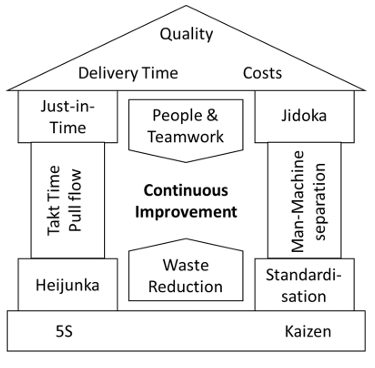
\includegraphics[width=\columnwidth]{HouseofToyota.png} 
        \caption{House of Toyota Manufacturing Systems from \cite{Impact_Lean_Prod}}
        \label{fig1:House of Toyota Manufacturing System}   
    \end{figure}
    \ref{fig1:House of Toyota Manufacturing System}
    
    Lean production is often given origin rights to Toyota production system. 5S, Kaizen, Just-in-Time, Continuous improvement, Standardisation etc. Where aim is to deliver produce while avoiding waste at the value chain. 
    
    The shown House of Lean Production is a symbol for the TPS principles. The triangle roof emlematizes the systamic focus on customer oriented key performance indicators (KPI) for quality, delivery time and cost. The basic approach is a continuous improvement of production. Industry 4.0 with IoT could bring lots of benefits within the Lean production standard. \cite{Impact_Lean_Prod}
    \newline\newline
    
    \section{Integration of Technologies}
    The concept of the Internet of Things is that everything is connected. Connecting expensive machines with expensive servers is not what is meant. But the things that are referenced are small microprocessors combined with sensors and actuators that could theoretically be made to collect and control anything. Making anything a part of the Internet (or intranet, more preferable). Temperature and humidity (TH) is something that in many processes affects results in manufacturing, and factories set up routines and may have machines that halt work if thresholds are reached. But thanks to cheap sensors, production could have an overview of the TH in all areas of production, and letting crucial processes subscribe to this information production could be halted, and the data could also be saved and analyzed in later quality assessment. A customer complaint could for the manufacturer be linked to bad TH, and the manufacturer could then have traceability on all serial numbers produced under the same circumstances. The ERP and MES systems may react instantly to the shift in TH and switch production focus for the day if the automatic systems for bringing TH to wanted levels are not successful. 
    \newline\newline
    Making the collection of data, actuating actions, and analyzing automatic cyber-physical systems emerges where the systems themselves are able to make decisions based on set algorithms. Adding on top of this, we have machine learning technologies that could further enhance decision-making for the systems. Big Data and analytics which is closely related to AI is a subjects within industry which the servey in \cite{Impact_Lean_Prod} sees highest possible impact on most areas in lean production. Out of 11 TPS principles Kaizen, Just-in-Time, Jidoka, Heijunka, Standardisation, Takt time, Waste reduction is impacted the most. 
    \begin{figure}
        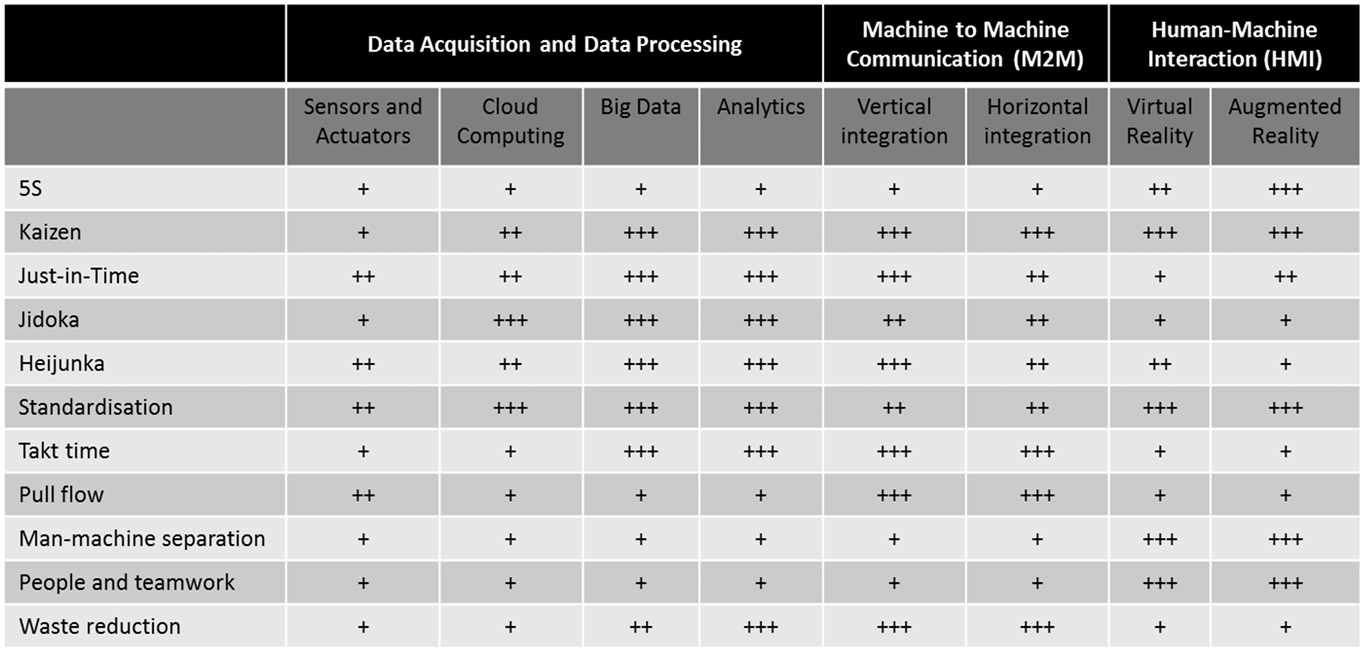
\includegraphics[width=\columnwidth]{ImpactMatrix.png} 
        \caption{Industry 4.0 impact matrix on lean production systems from \cite{Impact_Lean_Prod}}
        \label{fig2:Impact Matrix} 
    \end{figure}
    \ref{fig2:Impact Matrix}
    Another integration in lean production is virtual and augmented reality. Augmented reality could help operators to follow the lean production principles. Giving operators tips in their viewing field what to do and what to expect on a working station. THe augumented reality could have different levels with first level being for beginners giving clear instruction on what to do, what to expect on a station and when to consult a senior. To later levels where data is given upfront where a senior is able to decide what to do based on the data. AI in turn could be trained when being attached to a senior operator augumented reality. If the senior operator picks up a screwdriver. The augumented reality for a beginner operator will tell him/her to pick up the screwdriver. watching time to do different montagesteps could be recorded and AI could give tips based on this data to do montage in different steps. This are some examples why the industry accoring to \cite{Impact_Lean_Prod} sees highest impacts on lean principles 5S, Kaizen, Standardisation, Man-machine separation and teamwork. 
    \newline\newline
    5S is helped by our visuals highlighted on is something is missing. Likewise Standardisation is helped by these as operators differences in methods to produce is lowered when prompted how to do something compared to having an manual on the side that could be easier to avoid following. Kaizen (continuous improvement) is improved  when operators finds that given instruction och setup could be done faster if some setup is changed. Augmented reality could make it easier to visualise what changes to be done and also find out what montage steps that could be changed.  
    \newline\newline
    The systems, engeenering of systems and also implementation of systems. For example augumented reality is something that the article \cite{Change_Man_Landscape} discussed is hard to achieve for small and medium sized companies. The manpower with competence is not present enought. For this the article disussced collaboration and netwerking between industries is a way of sharing the burden of not having to invent the wheel in every factory site. 
\newline\newline
    Also the virtualization of factories is dependent on big engeenering force and complex software that is as above mentioned something that needs collaboration for small and medium sized companies. What in short is meant by virtualization is that the physical world is digitalization. In a way making it easier from a top down approach easier to monitor and find irregularities in the production process. 

    \section{Impact of efficiency and flexibility}
    The lean principles to reduce waste gets further backup by industry 4.0. A Use-case where Just-in-Time (JIT) gets improved by developing a JIT analyzing system where information about manufacturing orders, material deliveries, material stock and material consumption made it possible to send automatic purshasing orders to suppliers. Every material movement is monitored by sensors and posted into a database to be able to make analytics. When manufacturing machines brings down the material inventory to a dynamic minimum an automatic purchasing order is sent to supplier. The size of the purchasing order is calculated by an analytics service that use available information. Delivered material that in this system is tracked via a RFID system. The implementation of sensors and tracking RFID in the manufacturing process also gave benefits to traceability \cite{Impact_Lean_Prod} and process reliability which is other values in lean production. Getting traceability is a customer service that in my point of view, customers are willing to pay for and thereby extra value is added for manufacturer in the same time as a boarder type of customers are available.  
    \newline\newline
    Another example discussed in \cite{AugPCBA1}\cite{AugPCBA2} the usage of augumented reality for operator inspecting printed circuit board assemblies (PCBA). Normally today the operator is using a screen beside their reworking table. Before the physical PCBA is retrieved by the operator an automatic optical inspection (AOI) scanning has been conducted to find errors in soldering. The screen in usage highights the errors found in AOI for the operator to find on PCBA and fix. With augumented reality the operator get errors highlighted directly on board. Giving efficiency to operator not having to look back and forward between board and another screen. This solution uses a connection to the AOI system to get data so the augemented system in it self doesn't need to have optical detection capabilities.   
    
    
    \section{Challenges and Considerations}

    \section{Future Prospects}

    \section{Conclusion}


\printbibliography
\end{document}